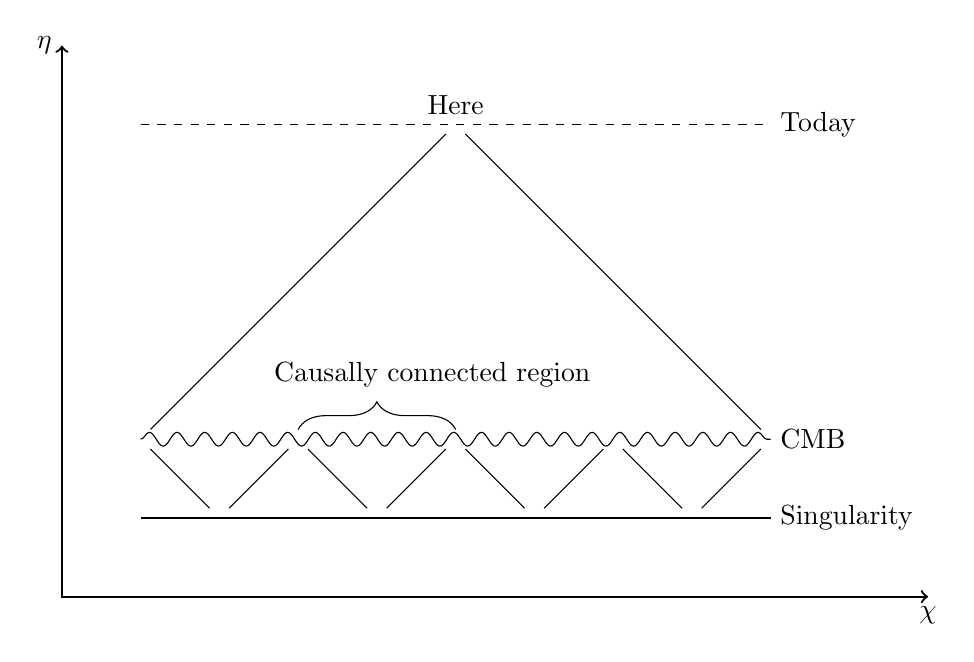
\begin{tikzpicture}
  \draw [<->,thick] (0,7) node (yaxis) [left] {$\eta$}
  |- (11,0) node (xaxis) [below] {$\chi$};

  % CMB

  % singularity
  \draw[] (1,1) -- (9,1) node [right] {Singularity};
  \draw[decorate,decoration=snake] (1,2) node (CMBl) {}  -- (9,2) node (CMBr) [right] {CMB};
  \draw[dashed] (1,6) -- (9,6) node [right] {Today};

  % causal contacts
  \draw (2,1) node (s1) {};
  \draw (4,1) node (s2) {};
  \draw (6,1) node (s3) {};
  \draw (8,1) node (s4) {};

  \draw (1,2) node (c1) {};
  \draw (3,2) node (c2) {};
  \draw (5,2) node (c3) {};
  \draw (7,2) node (c4) {};
  \draw (9,2) node (c5) {};
  \draw (5,6) node (now) {};

  
  \draw (c1) -- (s1) -- (c2);
  \draw (c2) -- (s2) -- (c3);
  \draw (c3) -- (s3) -- (c4);
  \draw (c4) -- (s4) -- (c5);

  \draw (c1) -- (now) -- (c5);
  \draw (now) node [above] {Here};

  \draw [decorate,decoration={brace,amplitude=10pt}]
  (c2.north) -- (c3.north) node [black,midway,yshift=20pt,xshift=20pt] {Causally connected region};

\end{tikzpicture}
